\documentclass[aspectratio=169, handout, t]{beamer}

%\usepackage[table]{xcolor}
\mode<presentation> {
\setbeamercovered{transparent}
  \usetheme{Boadilla}
\usepackage{booktabs}
%  \usetheme{Pittsburgh}
%\usefonttheme[2]{sans}
\renewcommand{\familydefault}{cmss}
%\usepackage{lmodern}
%\usepackage[T1]{fontenc}
%\usepackage{palatino}
%\usepackage{cmbright}

\useinnertheme{rectangles}
}
\usepackage{bm}
\usepackage{amsmath}
\usepackage{stackrel}
\setbeamercolor{normal text}{fg=black}
\setbeamercolor{structure}{fg= blue}
\definecolor{trial}{cmyk}{1,0,0, 0}
\definecolor{trial2}{cmyk}{0.00,0,1, 0}
\definecolor{darkgreen}{rgb}{0,.4, 0.1}
\usepackage{array}
 \usepackage{listings}
\definecolor{darkpurple}{rgb}{0.4, 0, 0.6}
\beamertemplatesolidbackgroundcolor{white}  \setbeamercolor{alerted
text}{fg=darkpurple}
\usepackage{tcolorbox}
\setbeamertemplate{caption}[numbered]\newcounter{mylastframe}

\font\domino=domino
\def\die#1{{\domino#1}}
\usepackage{tikz}
\usetikzlibrary{arrows}
\usepackage{colortbl}
\renewcommand{\familydefault}{cmss}
%\usepackage[all]{xy}

\usepackage{lipsum}

 \newenvironment{changemargin}[3]{%
 \begin{list}{}{%
 \setlength{\topsep}{0pt}%
 \setlength{\leftmargin}{#1}%
 \setlength{\rightmargin}{#2}%
 \setlength{\topmargin}{#3}%
 \setlength{\listparindent}{\parindent}%
 \setlength{\itemindent}{\parindent}%
 \setlength{\parsep}{\parskip}%
 }%
\item[]}{\end{list}}
\usetikzlibrary{arrows}

\usecolortheme{lily}

\newtheorem{com}{Comment}
\newtheorem{lem} {Lemma}
\newtheorem{prop}{Proposition}
\newtheorem{condition}{Condition}
\newtheorem{thm}{Theorem}
\newtheorem{defn}{Definition}
\newtheorem{cor}{Corollary}
\newtheorem{obs}{Observation}
 \numberwithin{equation}{section}

\makeatletter
\def\beamerorig@set@color{%
  \pdfliteral{\current@color}%
  \aftergroup\reset@color
}
\def\beamerorig@reset@color{\pdfliteral{\current@color}}
\makeatother

% Define the color and style for the code block
\usepackage{color}
\definecolor{codegreen}{rgb}{0,0.6,0}
\definecolor{codegray}{rgb}{0.5,0.5,0.5}
\definecolor{codepurple}{rgb}{0.58,0,0.82}
\definecolor{backcolour}{rgb}{0.95,0.95,0.92}

\lstdefinestyle{mystyle}{
    backgroundcolor=\color{backcolour},
    commentstyle=\color{codegreen},
    keywordstyle=\color{magenta},
    numberstyle=\tiny\color{codegray},
    stringstyle=\color{codepurple},
    basicstyle=\ttfamily\footnotesize,
    breakatwhitespace=false,
    breaklines=true,
    captionpos=b,
    keepspaces=true,
    numbers=left,
    numbersep=5pt,
    showspaces=false,
    showstringspaces=false,
    showtabs=false,
    tabsize=2
}

\lstset{style=mystyle}
\setbeamertemplate{navigation symbols}{}

\useoutertheme{miniframes}
\title[PLSC 30700]{Linear Models: CEF and Best Linear Predictor}

\author{Robert Gulotty}
\institute[Chicago]{University of Chicago}
\vspace{0.3in}


\begin{document}


\begin{frame}
\maketitle
\end{frame}


\begin{frame}{Populations, Projections, and Structure}
\begin{itemize}
\item Today we study relationships between random variables 
      $Y$ and $X = (X_1, \ldots, X_k)$ in the population.

\item The \textbf{Conditional Expectation Function (CEF)}:
      $m(X) = \mathbb{E}[Y \mid X]$.
      \\ \quad A potentially non-linear expectation of $Y$ based on $X$.

\item The \textbf{Best Linear Predictor (BLP)}:
      $\beta^* = \arg\min_b \mathbb{E}[(Y - X'b)^2]$.
      \\ \quad The linear projection of $Y$ onto $X$ in the population.

\item Later we will use algebra to fit a line in the sample and use probability theory to estimate the BLP.

\item Structural (exogeneity) assumptions determine whether the BLP coincides with the CEF.
\end{itemize}
\end{frame}




%%%%%%%%%%%%%%%%%%%%%%%%%%%%%%%%%%%%%%%%%%%%%%%%%%%%%%%%%%%%%%%%
\section{CEF}
%%%%%%%%%%%%%%%%%%%%%%%%%%%%%%%%%%%%%%%%%%%%%%%%%%%%%%%%%%%%%%%%

\begin{frame}{Properties of Conditional Expectation}
\begin{itemize}
  \item $m(X) \equiv \mathbb{E}[Y \mid X]$ \hfill (Definition)
  \item[*] Note: $\mathbb{E}[Y|X]$ is a random variable (a function of $X$), not a number!
  \bigskip
  \item $\mathbb{E}[\mathbb{E}[Y \mid X] \mid X] = \mathbb{E}[Y \mid X]$ \hfill (Idempotence)
  \bigskip
  \item $\mathbb{E}[\mathbb{E}[Y \mid X]] = \mathbb{E}[Y]$ \hfill (Law of Iterated Expectations)
  \bigskip
  \item $m(X) = \arg\min_{g} \mathbb{E}[(Y - g(X))^2]$ \hfill (Best predictor of $Y$ using $X$)

\end{itemize}
\end{frame}


\begin{frame}{CEF Error and Mean Independence}
\begin{itemize}
\item Define the CEF error: $e=Y-m(X)$, so $Y=m(X)+e$.
\item The CEF error has conditional mean zero (by construction):
\begin{align*}
\mathbb{E}[e|X]&=\mathbb{E}[Y-m(X)|X]=m(X)-m(X)=0
\end{align*}
\item And unconditional mean zero (by LIE):
\begin{align*}
\mathbb{E}[e]&=\mathbb{E}[\mathbb{E}[e|X]]=0
\end{align*}
\item $\mathbb{E}[e|X]=0$ is called \emph{mean independence}---true by construction, this is \textbf{not} full independence.
\end{itemize}
\end{frame}


\begin{frame}{Hansen Theorem 2.4: Properties of the CEF Error $e$}
\begin{enumerate}
\item $\mathbb{E}[e|X]=0$
\item $\mathbb{E}[e]=0$
\item If the rth moment of Y exists, the rth moment of $e$ exists. [Technical]
\item For \emph{any measurable function} h(X) where the expected product with $e$ exists [$\mathbb{E}[|h(X)e|]< \infty$], then, $\mathbb{E}[h(X)e]=0$
\end{enumerate}
\bigskip

\begin{tcolorbox}[colback=blue!5, colframe=blue!50, title=Key Point]
These are properties, not assumptions; they follow from LIE and the definition of the CEF: \alert{these properties are why we use the CEF as a mathematical tool.}
\end{tcolorbox}
\end{frame}



\begin{frame}{Why Covariance Matters for Decomposition}
Suppose we decompose a random variable into two parts: $Y = S + N$ (``signal'' + ``noise'').
\pause
\medskip

The variance of the sum is:
$$\operatorname{Var}(Y)=\operatorname{Var}(S)+\operatorname{Var}(N)+2\operatorname{Cov}(S,N)$$
\pause
\begin{itemize}
\item If $\operatorname{Cov}(S,N)\neq 0$, there is no clean separation: signal and noise share variation, and we cannot attribute variance to one or the other.
\pause
\item If $\operatorname{Cov}(S,N)= 0$, we get a \textbf{clean ANOVA-style decomposition}:
$$\operatorname{Var}(Y)=\operatorname{Var}(S)+\operatorname{Var}(N)$$
\end{itemize}
\pause
\medskip
\textbf{Question:} Is there a function of $X$ that decomposes $Y$ into uncorrelated signal and noise?
\end{frame}

\begin{frame}{Covariance of CEF and Its Error}
Yes---the CEF does exactly this.  Since $e$ is a random variable, compute its covariance with $m(X)$:
\begin{align*}
\mathbb{E}[e\, m(X)] & =  \mathbb{E}[\mathbb{E}[e\, m(X)|X]]=\mathbb{E}[m(X)\,\mathbb{E}[e|X]]=\mathbb{E}[m(X)\cdot 0]=0
\end{align*}\pause
Because $m(X)$ is a measurable function of $X$, Theorem 2.4.4 applies.\pause
\begin{align*}
\operatorname{Cov}(e , m(X)) & =  \mathbb{E}[e\, m(X)]- \mathbb{E}[e]\,\mathbb{E}[m(X)]=0- 0\cdot\mathbb{E}[m(X)]=0
\end{align*}\pause
So the \textbf{CEF decomposition} gives us exactly the clean split we wanted:
$$\operatorname{Var}(Y)=\operatorname{Var}(m(X))+\operatorname{Var}(e)$$
\end{frame}

\begin{frame}{Why Orthogonality? The Projection Interpretation}
This is not a mathematical coincidence.  It follows from what the CEF \emph{is}:

\begin{itemize}
\item The CEF minimizes $\mathbb{E}[(Y - g(X))^2]$ over \textbf{all} functions of $X$ (Thm 2.7).
\item In the language of Hilbert spaces, $m(X)$ is the \textbf{orthogonal projection} of $Y$ onto the space of all square-integrable functions of $X$.
\pause
\item A defining property of orthogonal projection: \alert{the residual is perpendicular to the space you project onto}.
\pause
\item Since $m(X)$, $X$, $X^2$, $\sin(X)$, \ldots\ are all in that space, the error $e$ must be uncorrelated with \emph{every} function of $X$.
\end{itemize}
\pause
\medskip
\begin{tcolorbox}[colback=blue!5, colframe=blue!50]
The CEF decomposition $\operatorname{Var}(Y)=\operatorname{Var}(m(X))+\operatorname{Var}(e)$ is a Pythagorean theorem: it holds because signal and noise are orthogonal.
\end{tcolorbox}
\end{frame}


\begin{frame}{Visualizing Projection in $L^2$ Space}
\begin{center}
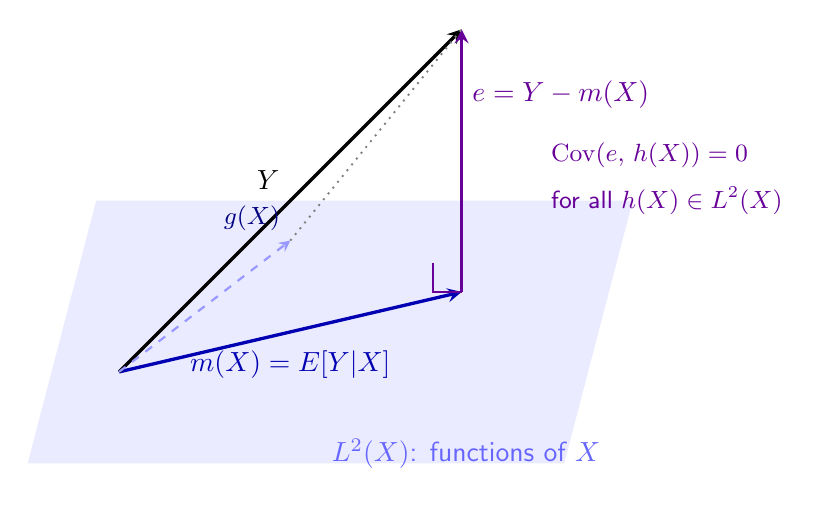
\begin{tikzpicture}[scale=1.45, >=stealth]
  % The subspace of functions of X (a plane through the origin)
  \fill[blue!8] (-0.5,-0.3) -- (4.2,-0.3) -- (4.8,2.0) -- (0.1,2.0) -- cycle;
  \node[blue!60, anchor=north east] at (4.6,0.0) {$L^2(X)$: functions of $X$};

  % Origin
  \coordinate (O) at (0.3,0.5);

  % The CEF m(X) -- a vector in the subspace
  \coordinate (mX) at (3.3,1.2);
  \draw[->, thick, blue!70!black, line width=1.2pt] (O) -- (mX)
    node[midway, below=3pt, blue!70!black] {$m(X) = \mathbb{E}[Y|X]$};

  % Y -- a vector outside the subspace
  \coordinate (Y) at (3.3,3.5);
  \draw[->, thick, black, line width=1.2pt] (O) -- (Y)
    node[midway, above left] {$Y$};

  % The error e = Y - m(X): vertical arrow from m(X) to Y
  \draw[->, thick, darkpurple, line width=1.2pt] (mX) -- (Y)
    node[pos=0.75, right, darkpurple] {$e = Y - m(X)$};

  % Right angle mark
  \draw[darkpurple, line width=0.8pt] (3.3,1.2) -- (3.05,1.2) -- (3.05,1.45);

  % Some other function g(X) in the subspace
  \coordinate (gX) at (1.8,1.65);
  \draw[->, thick, blue!40, line width=0.8pt, dashed] (O) -- (gX)
    node[above left, blue!50!black, font=\small] {$g(X)$};

  % Dotted line from g(X) to Y to show longer distance
  \draw[dotted, gray, line width=0.7pt] (gX) -- (Y);

  % Label the right angle as orthogonality
  \node[darkpurple, font=\small, anchor=west] at (4.0,2.4) {$\operatorname{Cov}(e,\, h(X))=0$};
  \node[darkpurple, font=\small, anchor=west] at (4.0,2.0) {for all $h(X) \in L^2(X)$};
\end{tikzpicture}
\end{center}
\vspace{-0.3cm}
The CEF is the closest point in $L^2(X)$ to $Y$.  The residual $e$ is orthogonal to the subspace.
\end{frame}


\begin{frame}{A Note on the Geometry}
The diagram on the previous slide is an \emph{analogy}, not a literal picture.  Random variables do not live in $\mathbb{R}^2$---they live in an abstract \textbf{Hilbert space} $L^2$.

\medskip
\begin{center}
\begin{tabular}{lll}
\toprule
\textbf{Euclidean $\mathbb{R}^n$} & & \textbf{Hilbert space $L^2$}\\
\midrule
Vector $\mathbf{v}$ & $\longleftrightarrow$ & Random variable $Y$\\
Dot product $\mathbf{u}\cdot\mathbf{v}$ & $\longleftrightarrow$ & $\mathbb{E}[UV]$ (inner product)\\
Length $\|\mathbf{v}\|^2$ & $\longleftrightarrow$ & $\mathbb{E}[Y^2]$ (second moment)\\
Perpendicularity $\mathbf{u}\cdot\mathbf{v}=0$ & $\longleftrightarrow$ & Orthogonality $\mathbb{E}[UV]=0$\\
Projection onto subspace & $\longleftrightarrow$ & Conditional expectation\\
\bottomrule
\end{tabular}
\end{center}

\medskip\pause
You do \emph{not} need to know Hilbert space theory for this course.  The takeaway is just the intuition: \alert{projection $\Rightarrow$ orthogonal residual $\Rightarrow$ clean variance decomposition}.
\end{frame}


\begin{frame}{How Much Does the CEF Leave Unexplained?}

The CEF $m(X)$ captures the systematic part of $Y$.  The error $e = Y - m(X)$ is everything else.

\medskip
\textbf{Unconditional error variance:}
$$\sigma^2 \equiv \operatorname{Var}[e]=\mathbb{E}[e^2]$$
The average prediction error across all values of $X$.

\medskip\pause
\textbf{Conditional error variance:}
$$\sigma^2(x)=\operatorname{Var}[e|X=x]=\mathbb{E}[e^2|X=x]$$
How uncertain is our prediction \emph{for a specific} $X=x$?\quad Averaging: $\sigma^2=\mathbb{E}[\sigma^2(X)]$.

\medskip\pause
\textbf{Example:} Predict vote share from incumbency.  $\sigma^2(D{=}1)$ may differ from $\sigma^2(D{=}0)$---incumbents might have more predictable outcomes than challengers.
\end{frame}


\begin{frame}{Mean-Variance Representation}
Define $u=\frac{e}{\sigma(X)}$, so $\mathbb{E}[u|X]=0$ and $\operatorname{Var}[u|X]=1$.  Then:
\begin{align*}
Y&=m(X)+\sigma(X)\, u
\end{align*}
\pause
$X$ matters in \textbf{two ways}:
\begin{itemize}
\item Through the \textbf{mean}: $m(X)$ shifts the expected outcome.
\item Through the \textbf{variance}: $\sigma(X)$ scales the noise.
\end{itemize}

\bigskip\pause
If $\sigma(X)$ is constant across all $X$: \textbf{homoskedastic} errors.\\
If $\sigma(X)$ varies with $X$: \textbf{heteroskedastic} errors.

\bigskip\pause
\textbf{Example:} In a model of household income, $\sigma(\text{Education})$ tends to increase with education---PhDs can be professors or hedge fund managers, while high-school graduates have a narrower income range.
\end{frame}


\begin{frame}{Hansen Theorem 2.6}
\begin{tcolorbox}[colback=blue!5, colframe=blue!50, title=Theorem 2.6 (More Variables Reduce Error Variance)]
Let $e_1=Y-m(X_1)$ and $e_{12}=Y-m(X_1, X_2)$.  Then:
$$\operatorname{Var}[Y]\geq \operatorname{Var}[e_1]\geq \operatorname{Var}[e_{12}]$$
\end{tcolorbox}
\smallskip
You will always explain (weakly) more of the variance with more variables.
This is why $R^2$ is a poor measure of model fit.

\smallskip\pause
\textbf{Proof strategy:} Show $\operatorname{Var}[m(X_1)] \leq \operatorname{Var}[m(X_1,X_2)]$---the finer CEF has (weakly) larger variance.  Then the \textbf{CEF decomposition}
$\operatorname{Var}[Y] = \operatorname{Var}[m(X)] + \mathbb{E}[\operatorname{Var}[Y|X]]$
converts this into the result about error variances.
\end{frame}

\begin{frame}{Proof of Theorem 2.6: Setup}
\textbf{Goal:} Show $\mathbb{E}[m(X_1)^2] \leq \mathbb{E}[m(X_1,X_2)^2]$, where $m(\cdot)$ denotes the relevant CEF.\\ \medskip\pause
\textbf{Step 1.} By LIE, the coarser CEF is a conditional expectation of the finer one:
$$m(X_1) \;=\; \mathbb{E}[Y|X_1] \;=\; \mathbb{E}\!\big[\,\mathbb{E}[Y|X_1,X_2]\;\big|\;X_1\big] \;=\; \mathbb{E}\!\big[\,m(X_1,X_2)\;\big|\;X_1\big]$$
\pause
\textbf{Step 2.} Jensen's inequality: for any convex function $\varphi$ (such as $z\mapsto z^2$),
$$\varphi\!\big(\mathbb{E}[Z|X_1]\big) \;\leq\; \mathbb{E}\!\big[\varphi(Z)\;\big|\;X_1\big]$$
\pause
Apply with $Z = m(X_1,X_2)$ and $\varphi(z)=z^2$:
$$\Big(\mathbb{E}\!\big[m(X_1,X_2)\;\big|\;X_1\big]\Big)^{\!2} \;\leq\; \mathbb{E}\!\big[m(X_1,X_2)^2\;\big|\;X_1\big]$$
\pause
The left side is $m(X_1)^2$ by Step 1, so:
$$m(X_1)^2 \;\leq\; \mathbb{E}\!\big[m(X_1,X_2)^2\;\big|\;X_1\big]$$
\end{frame}

\begin{frame}{Proof of Theorem 2.6: Conclusion}
\textbf{Step 3.} Take unconditional expectations of both sides:
$$\mathbb{E}\!\big[m(X_1)^2\big] \;\leq\; \mathbb{E}\!\big[m(X_1,X_2)^2\big]$$
\pause
\textbf{Step 4.} Convert to variances. Recall $\operatorname{Var}[Z]=\mathbb{E}[Z^2]-(\mathbb{E}[Z])^2$, and by LIE:
$$\mathbb{E}[m(X_1)]=\mathbb{E}[m(X_1,X_2)]=\mathbb{E}[Y]$$
so $(\mathbb{E}[Z])^2$ is the same for both.  Subtracting it from the inequality above:
$$\operatorname{Var}[m(X_1)] \;\leq\; \operatorname{Var}[m(X_1,X_2)]$$
\pause
\textbf{Step 5.} Since $\operatorname{Var}[Y]=\operatorname{Var}[m]+\operatorname{Var}[e]$ (by the CEF decomposition), larger $\operatorname{Var}[m]$ means smaller $\operatorname{Var}[e]$:
$$\operatorname{Var}[e_1] \;\geq\; \operatorname{Var}[e_{12}] \qquad \square$$
\end{frame}


\begin{frame}{Hansen Theorem 2.7: CEF as Best Predictor}
\begin{tcolorbox}[colback=blue!5, colframe=blue!50, title=Theorem 2.7 (CEF Is the Best Predictor), boxsep=2pt, top=2pt, bottom=2pt]
If $\mathbb{E}[Y^2]<\infty$, then for any measurable function $g(X)$:
$\mathbb{E}\!\left[(Y-m(X))^2\right] \leq \mathbb{E}\!\left[(Y-g(X))^2\right]$.
The CEF $m(X)=\mathbb{E}[Y|X]$ minimizes mean squared prediction error.
\end{tcolorbox}
\vspace{-4pt}
{\small\textbf{Proof:}}\pause
{\footnotesize
\begin{align*}
\mathbb{E}\!\left[(Y-g(X))^2\right]&=\mathbb{E}\!\left[(e+m(X)-g(X))^2\right] \tag{$Y= e+m(X)$}\\ \pause
&=\mathbb{E}[e^2]+2\mathbb{E}[e(m(X)-g(X))]+\mathbb{E}[(m(X)-g(X))^2]\\\pause
 &=\mathbb{E}[e^2]+0+\mathbb{E}[(m(X)-g(X))^2] \tag{by thm 2.4.4}\\\pause
  &\geq \mathbb{E}[e^2] = \mathbb{E}[(Y-m(X))^2] \tag{squares $\geq 0$}
 \end{align*}}
\end{frame}


\begin{frame}{Implications of Theorem 2.7}
\begin{itemize}
\item Regardless of the distribution of $X$ and $Y$, the best predictor is the CEF $m(X)$.
\begin{itemize}
\item For example: Consider the intercept only model $\mu=\mathbb{E}[Y]$.
\item The best predictor for $Y$, among constants, is $\mu$.
\end{itemize}
\item Since the CEF is the best predictor, anything else must be identical or worse.
\item We don't know what the joint distribution is, so we don't generally know the CEF, we have to use an estimator.
\end{itemize}
\end{frame}

\begin{frame}{Linear CEF and Best Prediction}

If $m(X)$ is \emph{linear} in $X=(X_1,\ldots,X_k,1)'$, we can write $m(X)=X'\beta$.  The \textbf{linear regression model} is:
\begin{align*}
Y&=X'\beta+e, \quad \mathbb{E}[e|X]=0
\end{align*}
If homoskedastic: $\mathbb{E}[e^2|X]=\sigma^2$.\\
\bigskip\pause
\textbf{Best prediction property:}
\begin{itemize}
\item If the CEF is linear, the solution to $\beta=\arg \min_b \mathbb{E}[(Y-X'b)^2]$ gives the right formula for $\beta$.
\item If the CEF is nonlinear, the solution gives the best linear approximation to the true CEF.
\end{itemize}
\end{frame}

\begin{frame}{From CEF to Linear Predictors}
\begin{itemize}
\item The CEF provides: summarization, MMSE prediction, and ANOVA decomposition.\pause
\item But the CEF requires knowing the conditional distribution $f_{Y|x}(y|x)$.
\begin{itemize}
\item Exception: CEF is always linear if X is discrete and all interactions are included.
\end{itemize}\pause
\item We will instead approximate the CEF using a \textbf{Best Linear Predictor} (BLP).
\item Later we will show that OLS estimates are optimal \textbf{if} the CEF is linear and the residuals are homoskedastic.
\end{itemize}
\end{frame}

\begin{frame}{The CEF in Political Science}
\begin{itemize}
\item \textbf{Voter turnout and age:} $\mathbb{E}[\text{Turnout}|\text{Age}]$ is nonlinear---turnout rises steeply from 18--30, plateaus in middle age, and rises again among retirees.\pause
\item \textbf{Income and party ID:} $\mathbb{E}[\text{Income}|\text{Party}]$ differs across categories---the CEF is just group means when $X$ is discrete.\pause
\item \textbf{Conflict and GDP:} $\mathbb{E}[\text{Conflict}|\text{GDP}]$ may be highly nonlinear, with sharp thresholds at low GDP.
\end{itemize}
\bigskip
\textbf{Takeaway:} The CEF is the target. But when the relationship is complex, we approximate it with a linear predictor and interpret accordingly.
\end{frame}

\begin{frame}{What Have We Learned About the CEF?}
\begin{tcolorbox}[colback=blue!5, colframe=blue!50, title=CEF Summary]
\begin{enumerate}
\item $m(X)=\mathbb{E}[Y|X]$ is the \textbf{best predictor} of $Y$ given $X$ (Thm 2.7).
\item The CEF error $e=Y-m(X)$ satisfies $\mathbb{E}[e|X]=0$ \textbf{by construction}---not an assumption (Thm 2.4).
\item Signal and noise are uncorrelated: $\text{Cov}(m(X), e)=0$.
\item More variables $\Rightarrow$ (weakly) smaller error variance (Thm 2.6).
\item $Y = m(X) + \sigma(X)u$: $X$ shapes both the mean \emph{and} the variance.
\end{enumerate}
\end{tcolorbox}
\medskip
\textbf{Next:} We approximate $m(X)$ with a \emph{linear} function---the Best Linear Predictor.
\end{frame}

%%%%%%%%%%%%%%%%%%%%%%%%%%%%%%%%%%%%%%%%%%%%%%%%%%%%%%%%%%%%%%%%
\section{Linear Predictors}
%%%%%%%%%%%%%%%%%%%%%%%%%%%%%%%%%%%%%%%%%%%%%%%%%%%%%%%%%%%%%%%%

\begin{frame}{(Best) Linear Predictors (bivariate case)}

\begin{itemize}
\item Suppose we want a predictor $ \mathbb{E}^{*}(Y|X)$ that is \textbf{linear}:
$$f(X)=a+bX$$\pause
Our standard for prediction is to minimize the mean-square error (best): \\
\item Whereas the CEF might be infinitely complex, the BLP is characterized just by two numbers, $a$ and $b$.\\
\pause
Choose $a$ and $b$ to minimize
$$M= \mathbb{E}[(Y-(a+bX))^2]$$
\end{itemize}
\end{frame}

\begin{frame}{Solving for Best Linear Predictor ($a$ and $b$)}
\textbf{FOC w.r.t.\ $a$:}\pause
\begin{align*}
0&=  -2 \mathbb{E}[Y]+2 \mathbb{E}[a+bX] \implies a= \mathbb{E}[Y]-b \mathbb{E}[X]
\end{align*}
\pause
\textbf{FOC w.r.t.\ $b$:}\pause
\begin{align*}
0&= -2 \mathbb{E}[YX]+2 \mathbb{E}[(a+bX)(X)]\\
 \mathbb{E}[YX]&= [ \mathbb{E}[Y]-b \mathbb{E}[X]] \mathbb{E}[X]+b \mathbb{E}[X^2]\\\pause
 \mathbb{E}[YX]- \mathbb{E}[Y]\mathbb{E}[X]&= b[ \mathbb{E}[X^2]- \mathbb{E}[X]^2]\\\pause
b&=\frac{Cov(X,Y)}{Var(X)}\\
\end{align*}
\end{frame}


\begin{frame}{Best Linear Predictor}
The best linear predictor is the population linear projection:
\begin{align*}
 \mathbb{E}^{*}[Y|X]&=\beta_0+\beta_1X\\ \pause
Y&=\beta_0+\beta_1X+e
\end{align*}
\pause
\begin{itemize}
\item Parameters (in Greek)
\begin{itemize}
\item The slope $\beta =\frac{Cov(X,Y)}{Var(X)}$
\item The intercept $\alpha=\mathbb{E}(Y)-\beta \mathbb{E}(X)$
\end{itemize}
\item $\mathcal{P}(Y|X)= \mathbb{E}[Y]+\frac{\text{Cov}(X,Y)}{\text{Var}(X)}\cdot(X-\mathbb{E}[X])$
\end{itemize}
\end{frame}




\begin{frame}{Deriving Variance of BLP at Minimized Values}
\begin{align*}
\beta &=\frac{Cov(X,Y)}{Var(X)}&&  \beta Var(X)=Cov(X,Y)
\end{align*}  \pause
\begin{align*}
\mathbb{E}[(Y-(\alpha+\beta X))^2]-\mathbb{E}[Y-(\alpha+\beta X)]^2 &=Var(Y-(\alpha+\beta X))\\\pause
&=Var(Y-\beta X)\\\pause
&=Var(Y)+\beta^2Var(X)-2\beta Cov(X,Y)\\\pause
 &=Var(Y)+\beta^2Var(X)-2\beta^2 Var(X)\\\pause
  &=Var(Y)-\beta^2 Var(X)\\\pause
  \sigma^2_\epsilon  &=\sigma^2_Y-\beta^2 \sigma^2_X\\
\end{align*}
\end{frame}



\begin{frame}{Example: Population Linear Projection is not the CEF}
Example: $Y=X+X^2$, $X\sim N(0,1)$, $\mathbb{E}[X]=\mathbb{E}[X^3]=0$, $\mathbb{E}[X^2]=1$\\
True CEF: $m(X)=X+X^2$\\
 Population Linear Projection: $Y=\alpha+\beta X+e$.
\begin{align*}
\alpha&=\mathbb{E}[Y]-\beta \mathbb{E}[X]=\mathbb{E}[X+X^2]-\beta\cdot 0=0+1-0\\
\beta&=\text{Cov}(X,Y)/\text{Var}(X)=\text{Cov}(X,X+X^2)/1=1/1\\
\mathcal{P}(Y|X)&=1+1*X\\\pause
e&=m(X)-\mathcal{P}(Y|X)=X^2-1\\
\mathbb{E}[eX]&=\mathbb{E}[(X^2-1)X]=\mathbb{E}[X^3-X]=0
\end{align*}
\pause
The BLP error $e=X^2-1$ is a function of $X$, so $\mathbb{E}[e|X]=X^2-1\neq 0$.

\smallskip
$\mathbb{E}[Xe]=0$ holds, but $\mathbb{E}[e|X]=0$ fails---the error has a systematic nonlinear pattern in $X$.  This is what ``weaker'' means: $\mathbb{E}[e|X]=0 \implies \mathbb{E}[Xe]=0$, but not vice versa.
\end{frame}



\begin{frame}{CEF vs Linear Predictors / Projection}
\begin{itemize}
\item CEF ($m(X)$)
\begin{itemize}
\item Best prediction, the prediction that minimizes squared error.
\item Can be non-linear.
\item Requires knowing joint distribution.
\item Prediction Errors are uncorrelated with any function of X. ($E(e|X)=0$.)
\end{itemize}

\item Linear Predictor/ Projection ($\mathcal{P}(Y|X)$)
\begin{itemize}
\item Draws a line (plane/hyperplane)
\item Requires knowing variances and covariances.
\item Prediction Errors are uncorrelated with X ($E(Xe)=0$.)
\end{itemize}
\end{itemize}
\end{frame}


\begin{frame}{CEF vs BLP: The Big Picture}
\begin{tcolorbox}[colback=blue!5, colframe=blue!50, title=Why Settle for Linear?]
\begin{itemize}
\item The CEF is the \emph{best possible} predictor---but we rarely know it.
\item The BLP is the best \emph{linear} predictor---and we only need $\text{Cov}(X,Y)$ and $\text{Var}(X)$.
\item When the CEF is actually linear (e.g., jointly normal $X,Y$), BLP $=$ CEF.
\item When the CEF is nonlinear, BLP gives the best linear approximation.
\end{itemize}
\end{tcolorbox}
\medskip\pause
\textbf{Key insight:}  $\mathbb{E}[Xe]=0$ (BLP errors uncorrelated with $X$) is \emph{weaker} than $\mathbb{E}[e|X]=0$ (CEF errors mean-independent of $X$).  The BLP projection ``uses up'' the linear information in $X$, but may leave nonlinear patterns in the residual.
\end{frame}


\begin{frame}{Why Write $\mathbb{E}[X_i e_i]=0$?}
\begin{itemize}
\item Saying ``$X$ is exogenous'' is intuitive but vague.  Writing $\mathbb{E}[X_i e_i]=0$ buys you three things:\pause
\begin{enumerate}
\item \textbf{It makes assumptions precise and testable.}  ``Exogenous'' could mean many things.  $\mathbb{E}[X_i e_i]=0$ says \emph{exactly} what must hold---and you can check whether the data are consistent with it.\pause
\item \textbf{It generalizes.}  Swap $X_i$ for an instrument $Z_i$ and you get IV: $\mathbb{E}[Z_i e_i]=0$.  Add more conditions and you get GMM.  Every estimator in this course is defined by \emph{which} moment conditions it solves.\pause
\item \textbf{It tells you what your estimator is doing.}  OLS finds the $\hat{\beta}$ that makes $\frac{1}{n}\sum X_i(Y_i - X_i'\hat{\beta})=0$.  The formula $(\bm{X}'\bm{X})^{-1}\bm{X}'\bm{Y}$ \emph{is} the solution to this system of equations.
\end{enumerate}
\end{itemize}
\end{frame}


\begin{frame}{From Theory to Moment Conditions: A Preview}
Every empirical model in this course follows the same logic:
\vspace{-2pt}
\begin{tcolorbox}[colback=blue!5, colframe=blue!50]
\begin{enumerate}
\item \textbf{Substantive claim:}  A mechanism, institution, or design feature creates a restriction on the data.
\item \textbf{Moment condition:}  Translate that claim into $\mathbb{E}[g(W_i, \theta)]=0$.
\item \textbf{Estimator:}  Find $\hat{\theta}$ that solves the sample analog.
\end{enumerate}
\end{tcolorbox}

\smallskip\pause
\textbf{Example:} In a randomized experiment, random assignment means potential outcomes are independent of treatment.  This implies $\mathbb{E}[D_i e_i]=0$, and OLS consistently estimates the ATE.

\smallskip\pause
\textbf{Counterexample:} If subjects self-select into treatment based on expected benefits, $\mathbb{E}[D_i e_i]\neq 0$.  OLS is inconsistent---you need a \emph{different} moment condition (e.g., from an instrument).
\textbf{The question is always:} \alert{Why should this moment condition hold?}
\end{frame}


\begin{frame}[fragile]{BLP in R: From Formula to Code}
\begin{lstlisting}[language=R]
# Population formula: beta = Cov(X,Y) / Var(X)
beta_formula <- cov(x, y) / var(x)
alpha_formula <- mean(y) - beta_formula * mean(x)

# OLS estimates the same thing from a sample
mod <- lm(y ~ x)
coef(mod)  # compare to c(alpha_formula, beta_formula)

# With multiple regressors: beta = solve(Q_XX) %*% Q_XY
X <- cbind(1, x1, x2)
beta_matrix <- solve(t(X) %*% X) %*% t(X) %*% y
coef(lm(y ~ x1 + x2))  # same answer
\end{lstlisting}
\end{frame}


%%%%%%%%%%%%%%%%%%%%%%%%%%%%%%%%%%%%%%%%%%%%%%%%%%%%%%%%%%%%%%%%
\section{Best Linear Predictor}
%%%%%%%%%%%%%%%%%%%%%%%%%%%%%%%%%%%%%%%%%%%%%%%%%%%%%%%%%%%%%%%%

\begin{frame}{From Bivariate to Multivariate Linear Prediction}
\begin{itemize}
\item So far we derived the BLP for a single regressor: $\beta = \text{Cov}(X,Y)/\text{Var}(X)$.
\item In practice, we want to predict $Y$ using \emph{many} variables: $X = (X_1, X_2, \ldots, X_k, 1)'$.
\item The algebra generalizes: scalar variances and covariances become \textbf{matrices}.
\end{itemize}
\bigskip\pause
\begin{defn}[Mean Square Prediction Error]
The \textbf{MSPE} of a linear predictor $X'\beta$ is:
$$S(\beta) = \mathbb{E}\!\left[(Y - X'\beta)^2\right]$$
This is the expected squared distance between $Y$ and our prediction.  The \textbf{best linear predictor} minimizes $S(\beta)$ over all $\beta \in \mathbb{R}^k$.
\end{defn}
\end{frame}

\begin{frame}{Regularity Conditions}
\begin{itemize}
\item Given $Y$ and $X=\begin{pmatrix} X_1\\ X_2\\X_3\\1 \end{pmatrix}$, we need three conditions for the BLP to exist:
\begin{enumerate}
\item $\mathbb{E}[Y^2]<\infty$ \hfill (finite second moment of $Y$)
\item $\mathbb{E}\|X\|^2<\infty$ \hfill (finite second moments of regressors)
\item $\mathbf{Q}_{XX}=\mathbb{E}[XX']$ is positive definite \hfill (no perfect collinearity)
\end{enumerate}\pause
\bigskip
\item Conditions 1--2 ensure $S(\beta)$ is finite.  Condition 3 ensures a \emph{unique} minimizer.
\item If $\mathbf{Q}_{XX}$ is not positive definite, some linear combination of regressors is constant---and the coefficients cannot be separately identified.
\end{itemize}
\end{frame}



\begin{frame}{Deriving the Linear Projection Coefficient $\beta$}
\begin{align*}
S(\beta)&=\mathbb{E}[(Y-X'\beta)(Y-X'\beta)]\\\pause
&=\mathbb{E}[Y^2]-2\beta'\mathbb{E}[XY]+\beta'\mathbb{E}[XX']\beta\\\pause
0&=\frac{\partial}{\partial \beta} S(\beta)=-2\mathbb{E}[XY]+2\mathbb{E}[XX']\beta\\\pause
\mathbf{Q}_{XY}&=\mathbf{Q}_{XX}\beta\\\pause
\mathbf{Q}_{XX}^{-1}\mathbf{Q}_{XY}&=\beta\\\pause
\mathbb{E}[XX']^{-1}\mathbb{E}[XY]&=\beta
\end{align*}
\end{frame}

\begin{frame}{Linear Projection and Projection Error}
\begin{align*}
\mathcal{P}[Y|X]&=X'\beta=X'\mathbb{E}[XX']^{-1}\mathbb{E}[XY]
\end{align*}\pause
The projection error is $e=Y-X'\beta$, so $Y=X'\beta+e$.\\
\medskip
The error is uncorrelated with $X$:
\begin{align*}
\mathbb{E}[Xe]&=\mathbb{E}[XY]-\mathbb{E}[XX']\mathbb{E}[XX']^{-1}\mathbb{E}[XY]=0\\
\begin{pmatrix}\mathbb{E}[X_1e]\\\mathbb{E}[X_2e] \\ \vdots \\\mathbb{E}[1*e] \end{pmatrix}&=\begin{pmatrix}0\\0\\ \vdots \\ 0\end{pmatrix}
\end{align*}
This is $k$ equations, the last of which is $\mathbb{E}[e]=0$ when there is a constant.
\end{frame}

\begin{frame}{What If There Is No Intercept?}
If $X$ does not include a constant, the moment conditions are only $\mathbb{E}[X_j e]=0$ for each regressor---there is no equation forcing $\mathbb{E}[e]=0$.
\pause

\medskip
\textbf{Consequences:}
\begin{itemize}
\item The projection line is forced through the origin: $\mathcal{P}[Y|X]=X'\beta$ with no intercept.
\item The error $e$ can have a nonzero mean: $\mathbb{E}[e]\neq 0$ in general.
\pause
\item The usual decomposition $\operatorname{Var}(Y)=\operatorname{Var}(X'\beta)+\operatorname{Var}(e)$ still holds (since $\mathbb{E}[Xe]=0$), but $\mathbb{E}[Y]\neq \mathbb{E}[X'\beta]$.
\end{itemize}
\pause
\medskip
\textbf{Takeaway:} Always include a constant unless you have a substantive reason not to.  Omitting it forces the regression through the origin and allows systematic over- or under-prediction on average.
\end{frame}

\begin{frame}{The Design Matrix}

$\beta = \mathbb{E}[XX']^{-1}\mathbb{E}[XY]$ exists and is unique \emph{if} $\mathbf{Q}_{XX}=\mathbb{E}[XX']$ is invertible.\\
\bigskip
$\mathbf{Q}_{XX}$ is the population second moment matrix of $X$.\\
\bigskip
For any non-zero $\alpha \in \mathbb{R}^k$
$$\alpha'\bm{Q}_{XX}\alpha=\mathbb{E}[\alpha'XX'\alpha]=\mathbb{E}[(\alpha'X)^2] \geq 0$$
This must be strictly $>0$ to be invertible, if not, there is no unique solution to $\mathbf{Q}_{XY}=\mathbf{Q}_{XX}\beta$, and we say $\beta$ is not identified.
\end{frame}


\begin{frame}{Application: Linear Probability Model (Binary $Y$)}
\begin{align*}
P(Y=1|X)&=\beta_0+\beta_1X
\end{align*}
\begin{itemize}
\item Suppose we have a binary outcome: $Y=\mathbb{I}(\omega\in B)$
\item $\beta_0$ is the probability that $Y=1$ if $X=0$
\item $\beta_1$ is the change in probability that $Y=1$ given a one unit change in $X$.
\item The BLP is still the best linear predictor: $\beta=\mathbb{E}[XX']^{-1}\mathbb{E}[XY]$.
\item However, it is an approximation to a probability, not itself a probability.
\end{itemize}
\end{frame}


\begin{frame}{Linear Predictor Error Variance}
\begin{itemize}
\item Hansen defines $\sigma^2=\mathbb{E}[e^2]$, $Q_{YY}=\mathbb{E}[Y^2]$ and $\mathbf{Q}_{YX}=\mathbb{E}[YX']$, a $1\times k$ vector.
\item Recall, $X$ and  $\beta$ are $k\times 1$ vectors.
\begin{align*}
\sigma^2&=\mathbb{E}[(Y-X'\beta)^2]\\ \pause
&=\mathbb{E}[Y^2]-2\mathbb{E}[YX']\beta+\beta'\mathbb{E}[XX']\beta\\\pause
&=Q_{YY}-2\bm{Q}_{YX}\bm{Q}^{-1}_{XX}\bm{Q}_{XY}+\bm{Q}_{YX}\bm{Q}^{-1}_{XX}\bm{Q}_{XX}\bm{Q}^{-1}_{XX}\bm{Q}_{XY}\\\pause
&=Q_{YY}-\bm{Q}_{YX}\bm{Q}^{-1}_{XX}\bm{Q}_{XY}\\\pause
&\equiv Q_{YY\cdot X}
\end{align*}
\end{itemize}
\end{frame}

\begin{frame}{Intercepts and Slopes}
\begin{itemize}
\item We will often exclude the 1 from X and write the linear projection as:
$$Y=X'\beta+\alpha+e$$
\item Demeaning we have a useful reinterpretation of the projection coefficient:
\begin{align*}
Y-\mu_Y&=(X-\mu_X)'\beta+e\\
\beta&=(\mathbb{E}[(X-\mu_X)(X-\mu_X)'])^{-1}\mathbb{E}[(X-\mu_X)(Y-\mu_Y)]\\
\beta&=var[X]^{-1}cov(X,Y)\\
\end{align*}
\end{itemize}
\end{frame}

%%%%%%%%%%%%%%%%%%%%%%%%%%%%%%%%%%%%%%%%%%%%%%%%%%%%%%%%%%%%%%%%
\section{Omitted Variable Bias}
%%%%%%%%%%%%%%%%%%%%%%%%%%%%%%%%%%%%%%%%%%%%%%%%%%%%%%%%%%%%%%%%

\begin{frame}{Partitions and Regression Sub-Vectors}
\begin{itemize}
\item Divide our regressors into $X=\begin{pmatrix} X_1\\ X_2\end{pmatrix}$, so the linear projection is:
\begin{align*}
Y&=X_1'\beta_1+X_2'\beta_2+e, \quad \mathbb{E}[Xe]=0
\end{align*}
\item We can partition $\mathbf{Q}_{XX}$ and $\mathbf{Q}_{XY}$:
\begin{align*}
\mathbf{Q}_{XX}&=\begin{bmatrix} \mathbf{Q}_{11} &\mathbf{Q}_{12}\\\mathbf{Q}_{21}&\mathbf{Q}_{22}\end{bmatrix} \quad
\mathbf{Q}_{XY}=\begin{bmatrix} \mathbf{Q}_{1Y}\\\mathbf{Q}_{2Y}\end{bmatrix}
\end{align*}
\end{itemize}
\end{frame}

\begin{frame}{A Useful Formula}
\begin{itemize}
\item Recall the error variance was: $Q_{YY\cdot X}\equiv Q_{YY}-\bm{Q}_{YX}\bm{Q}^{-1}_{XX}\bm{Q}_{XY}$
\item Analogously $\mathbf{Q}_{11\cdot 2}\equiv \mathbf{Q}_{11}-\bm{Q}_{12}\bm{Q}^{-1}_{22}\bm{Q}_{21}$,and $\mathbf{Q}_{22\cdot 1}\equiv \mathbf{Q}_{22}-\bm{Q}_{21}\bm{Q}^{-1}_{11}\bm{Q}_{12}$, etc.
\item In each case, $\mathbf{Q}_{a\cdot b}$ is the variation in $a$ not predicted by the linear projection of $b$.
\end{itemize}
\end{frame}

%
%\begin{frame}{Schur Complement}
%\begin{align}
%\bm{Mz}\equiv \begin{bmatrix} \bm{A} & \bm{B}\\\bm{C} & \bm{D}\end{bmatrix}\begin{bmatrix} x\\y\end{bmatrix}&=0 \iff \nonumber\\\pause
%\bm{A}x+\bm{B}y&=0 \\
%\bm{C}x+\bm{D}y&=0\\\pause
%-\bm{CA}^{-1}(\bm{A}x+\bm{B}y)&=0 \tag{Multiply (5.1) by $-\bm{CA}^{-1}$}\\\pause
%\bm{C}x+\bm{D}y-\bm{CA}^{-1}(\bm{A}x+\bm{B}y)&=0 \tag{Add to (5.2)}\\\pause
%(\bm{D}-\bm{CA}^{-1}\bm{B})y&=0 \nonumber
%\end{align}\pause
%$\bm{D}-\bm{CA}^{-1}\bm{B}$ is the Schur complement of $\bm{A}$ in $\bm{M}$.
%\end{frame}


\begin{frame}{Partitioned Matrix Inversion and Regression}
\begin{itemize}
\item By similar reasoning:
$$\bm{Q}_{XX}^{-1}=\begin{bmatrix} \mathbf{Q}_{11\cdot 2}^{-1} &-\mathbf{Q}_{11\cdot 2}^{-1}\mathbf{Q}_{12}\mathbf{Q}_{22}^{-1}\\ -\mathbf{Q}_{22\cdot 1}^{-1}\mathbf{Q}_{21}\mathbf{Q}_{11}^{-1}&\mathbf{Q}_{22\cdot 1}^{-1}\end{bmatrix}$$
\item As a result:
\begin{align*}
\begin{bmatrix}\beta_1\\\beta_2\end{bmatrix}&=\begin{bmatrix} \mathbf{Q}_{11\cdot 2}^{-1} \mathbf{Q}_{1Y\cdot 2}\\ \mathbf{Q}_{22\cdot 1}^{-1} \mathbf{Q}_{2Y\cdot 1} \end{bmatrix}
\end{align*}
\item We can use $\beta_1=\mathbf{Q}_{11\cdot 2}^{-1} \mathbf{Q}_{1Y\cdot 2}$ to understand multivariate regression.
\end{itemize}
\end{frame}

\begin{frame}{Interpreting Multivariate Regression}
\begin{itemize}
\item The multivariate projection equation is $Y=X_1'\beta_1+X_2'\beta_2+e$.
\item Decompose $X_1$ into the part predicted by $X_2$ and the part that is not:
$$X_1 = \underbrace{X_2'\gamma_2}_{\text{explained by }X_2} + \underbrace{u_1}_{\text{residual}}$$
\pause
\item $\beta_1$ is the projection of $Y$ onto $u_1$---the variation in $X_1$ that is \emph{unique} to $X_1$, not shared with $X_2$.
\pause
\item \textbf{Example:} Regress growth on democracy ($X_1$) and institutions ($X_2$).  $\beta_1$ captures the effect of democracy \emph{after removing} what institutions already explain about democracy.
\end{itemize}
\end{frame}

\begin{frame}{Demonstration: Iterated Projection}
Divide $X$ into a single variable in $X_1$, with all the other variables in $X_2$, so that
$$Y=X_1'\beta_1+X_2'\beta_2+e$$
Regress $X_1$ on $X_2$:
\begin{align*}
X_1&=X_2'\gamma_2+u_1\\
\mathbb{E}[X_2u_1]&=0\\
\gamma_2&=\mathbf{Q}_{22}^{-1} \mathbf{Q}_{21}\\
\mathbb{E}[u_1^2]&=\mathbf{Q}_{11\cdot 2}\\
\mathbb{E}[u_1Y]&=\mathbf{Q}_{1Y}-\mathbf{Q}_{12}\mathbf{Q}^{-1}_{22}\mathbf{Q}_{2Y}=\mathbf{Q}_{1Y\cdot2}\\
\beta_1&=\mathbf{Q}_{11\cdot 2}^{-1} \mathbf{Q}_{1Y\cdot 2}=\frac{\mathbb{E}[u_1Y]}{\mathbb{E}[u_1^2]}
\end{align*}
\end{frame}

\begin{frame}{Omitted Variable Bias}
\begin{itemize}
\item \textbf{Long regression}: $Y=X_1'\beta_1+X_2'\beta_2+e$. \quad \textbf{Short regression}: $Y=X_1'\gamma_1+u$.
\pause
\item Substitute the long into the short:
\begin{align*}
\gamma_1&=(\mathbb{E}[X_1X_1'])^{-1}\mathbb{E}[X_1Y]\\
&=(\mathbb{E}[X_1X_1'])^{-1}\mathbb{E}[X_1(X_1'\beta_1+X_2'\beta_2+e)]
=\beta_1+\underbrace{(\mathbb{E}[X_1X_1'])^{-1}\mathbb{E}[X_1X_2']}_{\Gamma_{12}}\beta_2
\end{align*}
\pause
\item $\Gamma_{12}$: coefficient from regressing $X_2$ on $X_1$ (the \textbf{association} between included and omitted).
\item \alert{Bias} $= \Gamma_{12}\beta_2$: product of \emph{how correlated} $X_1$ and $X_2$ are and \emph{how much $X_2$ matters} for $Y$.
\end{itemize}
\end{frame}


\begin{frame}{OVB is Not Solved by Adding Variables}
\begin{itemize}
\item Suppose $Y=X'\beta+e=X_1'\beta_1+X_2'\beta_2+X_3'\beta_3+e$
\item Suppose we cannot measure $X_3$.  Instead, we can choose either:
$$Y=X_1'\gamma_1+u_1$$
$$Y=X_1'\delta_1+X_2'\delta_2+u_2$$
\item $\gamma_1=\beta_1+\Gamma_{12}\beta_2+\Gamma_{13}\beta_3$.
\item $\delta_1=\beta_1+\Gamma_{13\cdot 2}\beta_3$.
\item Which is better depends on the signs and sizes of these terms!
\end{itemize}
\end{frame}


\begin{frame}{OVB in Practice: Does Democracy Cause Growth?}
\begin{itemize}
\item Barro (1996) regresses GDP growth on a democracy index:
$$\text{Growth}_i = \beta_1 \text{Democracy}_i + e_i$$
\item But countries that democratize also tend to have stronger property rights, higher education, and colonial histories that affect growth.\pause
\item The OVB formula tells us:
$$\gamma_1 = \beta_1 + \underbrace{\Gamma_{12}}_{\substack{\text{correlation of}\\\text{democracy with}\\\text{institutions}}}\underbrace{\beta_2}_{\substack{\text{effect of}\\\text{institutions}\\\text{on growth}}}$$\pause
\item If institutions are positively correlated with democracy ($\Gamma_{12}>0$) and positively affect growth ($\beta_2>0$), then $\gamma_1$ \alert{overstates} the effect of democracy.
\item Adding controls can help---but only if they reduce the bias term, not increase it.
\end{itemize}
\end{frame}


\begin{frame}{Where We Stand}
\small
\begin{tcolorbox}[colback=blue!5, colframe=blue!50, title=Recap: From Population to Practice]
\begin{enumerate}
\item \textbf{CEF} ($m(X)=\mathbb{E}[Y|X]$): Best predictor, but requires the full joint distribution.
\item \textbf{BLP} ($\mathcal{P}[Y|X]=X'\beta$): Best \emph{linear} predictor, requiring only means, variances, and covariances.
\item \textbf{Partitioned regression}: Each coefficient captures the effect of a variable \emph{after removing} what other variables predict.
\item \textbf{OVB}: Omitting a correlated variable biases coefficients; adding variables doesn't always help.
\end{enumerate}
\end{tcolorbox}
\medskip
\textbf{Next:} All of this is in the \emph{population}. Starting next lecture, we move to \emph{samples}---using OLS to estimate $\beta$ and studying when OLS does a good job.
\end{frame}


\end{document}
